\documentclass[12pt,oneside,a4paper]{article}

\usepackage{./top/custom}

\lstset{language=Java}

\usepackage[backend=biber]{biblatex}
\addbibresource{./top/biblio.bib}

% Project related new commands
%%% restaurant types %%%
\newcommand{\Dish}[1][]{\lstinline|Dish|}
\newcommand{\Starter}{\lstinline|Starter|}
\newcommand{\MainDish}{\lstinline|MainDish|}
\newcommand{\Dessert}{\lstinline|Dessert|}
\newcommand{\Drink}{\lstinline|Drink|}
\newcommand{\Meal}{\lstinline|Meal|}
\newcommand{\HalfMeal}{\lstinline|HalfMeal|}
\newcommand{\FullMeal}{\lstinline|FullMeal|}
\newcommand{\Menu}[1][]{\lstinline|Menu|}
%%% user types %%%
\newcommand{\User}{\lstinline|User|}
\newcommand{\Courier}{\lstinline|Courier|}
\newcommand{\Customer}{\lstinline|Customer|}
\newcommand{\Manager}{\lstinline|Manager|}
\newcommand{\Restaurant}{\lstinline|Restaurant|}
%%% misc %%%
\newcommand{\Order}{\lstinline|Order|}
\newcommand{\Core}{\lstinline|Core|}
\newcommand{\MyFoodora}{\lstinline|MyFoodora|}
%% packages %%
\newcommand{\core}{\lstinline|core|}
\newcommand{\exceptions}{\lstinline|exceptions|}
\newcommand{\parsers}{\lstinline|parsers|}
\newcommand{\policies}{\lstinline|policies|}
\newcommand{\restaurantSetup}{\lstinline|restaurantSetup|}
\newcommand{\tests}{\lstinline|tests|}
\newcommand{\txtF}{\lstinline|txtFILES|}
\newcommand{\userI}{\lstinline|user_interface|}
\newcommand{\users}{\lstinline|users|}
%% clui %%
\newcommand{\Command}{\lstinline|Command|}
\newcommand{\CommandLine}{\lstinline|CommandLine|}
\newcommand{\CommandProcessor}{\lstinline|CommandProcessor|}
%% uml diagrams %%
\newcommand{\umld}{UML diagram : }


\begin{document}
\begin{titlepage}
\begin{center}


\includegraphics[scale=0.5]{./img/logo_centralesup.jpg} \hfill

\vfill 

\textsc{\Large IS1220 -- Object oriented Software design}\\[0.5cm]

\vfill

% Title
\HRule \\[0.4cm]
{ \LARGE \bfseries \textsc{MyFoodora}\\[0.4cm] }
\HRule \\[1.5cm]

{\Large 
1st part : the core system\\[0.1cm]
2nd part : the user interface\\[0.5cm]
}

\vfill

{\large
\begin{center}
  \textbf{Professor}\\[0.1cm]
  Paolo \textsc{Ballarini}
\end{center}
\vfill
\begin{center}
  \textbf{Authors}\\[0.1cm]
  John \textsc{de Wasseige}\\[0.1cm]
  Patrick \textsc{von Platen}
\end{center}
}

\vfill

{\large \today}

\end{center}
\end{titlepage}

\vspace*{5cm}
  
{\setlength{\parindent}{0pt}

  \textbf{What is new in part 2 ?}
  
  Some parts of the report have been modified and others added.

  More precisely, the introduction was slightly modified to
  tie in the updated report.
  Then a complete section~\ref{sec:user_interface} on
  the implementation of the user interfaces has been added.
  The results obtained when using both have been described in section~\ref{sec:results}.
  As we designed more classes, there are also new UML diagrams and code listings
  in the appendix.
  Finally, the conclusion has been updated to consider further work and
  make a general comment on the advantages and disadvantages of our solution.
  
}
\newpage

{\hypersetup{linkcolor=black}
\setcounter{tocdepth}{2}
\tableofcontents
}
\newpage

\section{Introduction} % (fold)
\label{sec:introduction}
Nowadays, more and more software programs are needed and designed every day.
They play an important role in everyday life and more specifically
in domains like ``\textit{manufacturing, banking, travel, communications,
defense, medicine, research, government, education, entertainement,
law, etc.}''\cite[p.6]{long2008critical}.
The goal of this project is to develop a software solution,
called \lstinline|MyFoodora|, whose functionality is similar to today's food delivery systems\footnote{such as \url{https://www.foodora.fr/}
and \url{https://deliveroo.fr/}.}.

We did not only want to create a program that \emph{works} under the given conditions,
but one that is \emph{resusable} and easily \emph{extendable}.
To meet our expectations, we applied \emph{design patterns} in order
to follow the well-known \emph{open/close principle}.
We thourougly thought and discussed which patterns to follow
and to implement before effectively writing down the code.
This brainstorming approach allowed us
\begin{enumerate}
  \item to keep a global overview of what was needed at which point and why,
  \item to acquire a good comprehension of the advantages and disadvantages of each
  design pattern.
\end{enumerate}

The implementation of the solution has not been done without \emph{difficulty}.
Basically, the main discussion was about the question to which point we needed to apply the
open/close principle and how to connect all components to the core system.
Applying the open/close principle requires indeed to write more code than 
needed if you just wanted to be ``locally efficient'' (with no 
intention to extend the code) and also often requires more data structures to assure a structured and closed transition of information between classes that is coherent everywhere.
Looking back, we can now say with certainty that those difficulties
led us to many discoveries in the~\textsc{Java} programming language.
We did not only learn ``new programming skills", but more importantly we really 
understood why certain methods, we saw in class earlier, are efficent and recommended to implement (using getters and setters f.e.). 

As the project is divided into two parts, the first being the \emph{core}
and the second the \emph{interface} of the \lstinline|MyFoodora| system,
this report presents at first only the guidelines of this first part's implementation but will later 
be extended for the second part as well.
A brief summary of the project's \emph{background} and \emph{requirements} will
be detailed in section~\ref{sec:background}.
Next, in section~\ref{sec:analysis_and_design}, we will first present
a general \emph{overview} and \emph{analysis} of our solution, second a detailed 
explanation of how and why the various design patterns are implemented.
The most interesting functions of our \emph{code} will then be
thoroughly detailed in section~\ref{sec:implementation}.
The different \emph{tests} we used along the implementation
and the \emph{results} obtained by our solution will respectively
be shown in sections~\ref{sec:testing} and~\ref{sec:results}.
Finally, section~\ref{sec:conclusion} will allow us to draw 
a \emph{conclusion} and consider \emph{further work}.

% section introduction (end) 
\newpage
\section{Background and requirements} % (fold)
\label{sec:background}

As already mentioned in the introduction, the project deals with the realisation of
a tool that simulates today's food delivery systems. The projet requires to have five main 
actors being the users: \Restaurant, \Customer, \Manager, \Courier~and the system (ie. the \Core).

A restaurant offers different \Meal, being either a \HalfMeal~or a  
\FullMeal. A \FullMeal~ is made of a \Starter, a \MainDish~and a \Dessert.
The \HalfMeal~consists of a \MainDish~and either a \Starter~or a \Dessert. 
Additionally each restaurant offers a \Menu~containing 
a list of \Starter, \MainDish~and \Dessert, so that a \Meal~can be chosen ``à la carte''. 

A \Customer~can choose one of three different \emph{fidelity card plans}
that allow him to some kind of reduction 
according to chosen \emph{fidelity card plan} \ref{sub:fidcardplan}.
All users contain basic attributes like a name, a surname, etc.
and have distinctive functions that are described 
in detail below in the ~\ref{sub:users}.
Moreover, the system implements different \emph{target profit policies},
\emph{delivery policies}, \emph{shipped order policies}
also being described in detail below \ref{sub:policies}.

Let's take a more detailed look at the requirements
needed for the core, the different actors,
the fidelity card plan and the supported policies.

\subsection{Core system} % (fold)
\label{sub:core_system}
\vspace{0.3\baselineskip}

\begin{itemize}
  \begin{minipage}{0.51\linewidth}
    \item setting of the service-fee
    \item setting of the markup percentage
    \item setting of the delivery cost
    \item notifying customers
  \end{minipage}
  \begin{minipage}{0.57\linewidth}
   \item allocating couriers to orders
   \item computing total income 
   \item choosing target profit policy
  \end{minipage}
\end{itemize}

% subsection core_system (end)

\subsection{Users} % (fold)
\label{sub:users}
\paragraph{Manager}~\vspace{0.3\baselineskip}
\begin{itemize}
  \begin{minipage}{0.47\linewidth}
    \item add/remove \User
    \item activate/deactivate \User
    \item profit related attribute
    \item income over period
    \item income per \Customer
  \end{minipage}
  \begin{minipage}{0.53\linewidth}
    \item target profit policy
    \item most selling \Restaurant
    \item most active \Courier
    \item setting delivery policy
  \end{minipage}
\end{itemize}

\paragraph*{Restaurant}~\vspace{0.3\baselineskip}
\begin{itemize}
  \begin{minipage}{0.47\linewidth}
    \item add/remove \Dish
    \item add/remove \Meal
    \item add/remove \Meal~of the week
  \end{minipage}
  \begin{minipage}{0.53\linewidth}
    \item set \lstinline|discountFactors|
    \item sort of shipped orders following policy
  \end{minipage}
\end{itemize}

\paragraph*{Customers}~\vspace{0.3\baselineskip}
\begin{itemize}
  \begin{minipage}{0.47\linewidth}
    \item place \Order
    \item choose fidelity plan option
    \item get history of orders
  \end{minipage}
  \begin{minipage}{0.53\linewidth}
    \item get info about fidelity plan and points
    \item access and modify account info
    \item give/remove consensus for notification
  \end{minipage}
\end{itemize}

\paragraph*{Couriers}~\vspace{0.3\baselineskip}
\begin{itemize}
  \begin{minipage}{0.47\linewidth}
    \item register/unregister their account
    \item set their state
  \end{minipage}
  \begin{minipage}{0.53\linewidth}
    \item change their position
    \item accept/refuse to a delivery call
  \end{minipage}
\end{itemize}

% subsection users (end)

\subsection{Policies} % (fold)
\label{sub:policies}
\paragraph{Target profit policies}~\vspace{0.3\baselineskip}
Two out of the three profit related quantities: \emph{service-fee,
the markup percentage, the delivery cost}
are taken as given inputs depending on the chosen \emph{target policy} as well as an expected profit.
The functions implemented by each policy allow the \Manager~to simulate the third 
profit related quantity that is not taken as an input and thus 
needed to achieve the profit. The profit is calculated as follows: 
\begin{center} 
  profit for one order = order price $\cdot$ markup percentage + service fee - delivery cost
\end{center}

\begin{itemize}
    \item \emph{targetProfit DeliveryCost}: the delivery cost is simulated.
    \item \emph{targetProfit ServiceFee}: the service fee is simulated.
    \item \emph{targetProfit Markup}: the markup percentage is simulated.
\end{itemize}

\paragraph{Delivery policies}~\vspace{0.3\baselineskip}
The delivery policies define in which way the \Core~choses the \Courier~for a placed \Order.

\begin{itemize}
    \item \emph{fastest delivery}: The courier having the shortest distance to the selected restaurant is chosen.
    \item \emph{fair-occupation delivery}: The courier having executed the least amount of orders is chosen.
\end{itemize}

\paragraph{Shipped order sorting policies}~\vspace{0.3\baselineskip}
The \emph{shipped order sorting policies} allow restaurants and managers
to sort the shipped orders according to different criterias.

\begin{itemize}
    \item \emph{most/least ordered Meal}: A ascending/descending list of all sold Meals
    \item \emph{most/least ordered dishes}: A ascending/descending list of all sold Dishes.
\end{itemize}

\paragraph{Fidelity Card Plan} 
\label{sub:fid_card_plan}

Each \Customer can choose between three different fidelity card plans having each different bonuses.

\begin{itemize}
  \item \emph{Basic fidelity card}: The \Customer has access to a special offer provided by each restaurant.
  \item \emph{Point fidelity card}: The \Customer collects fidelity points
  and gets a certain reduction after 
	having reached a certain limit of points.
	\item \emph{Lottery fidelity card}: The \Customer takes part in a lottery
  and has the chance of getting his order for free.
\end{itemize}

% subsection policies (end)

\subsection{Summary} % (fold)

In order to give a basic overview of the typical function, the ordering of a food item,
we want to briefly summarize this process.
A \Customer~will place an \Order~by choosing a one or more \Meal~or one or more \Dish~of a \Restaurant.
The \Order~containing all the necessary information is handed to the \Core.
The \Core~will treat the \Order~by choosing a \Courier~according to the \emph{Delivery policy}. 
The \Courier~can either accept or decline the \Order. If any \Courier~accepts the \Order,
it is executed and saved in the \Core.

% subsection summary (end)

% section background (end)
 
\newpage
\section{Analysis and design} % (fold)
\label{sec:analysis_and_design}
This section will describe the design of our solution and how
it meets the given requirements presented in section~\ref{sec:background}.
The first part will present the different \emph{design patterns}
used throughout the code.
These patterns are useful as they allow
\begin{enumerate}
  \item to avoid redesigning,
  \item to follow guidelines so that the solution is extendable,
  \item to isolate parts of the code that might undergo changes.
\end{enumerate}

\subsection{Factory pattern for \texttt{Dish} and \texttt{Meal} classes} % (fold)
\label{sub:factory_pattern_for_the_texttt_dish_and_texttt_meal_classes}
When going through the different requirements for the two classes, a first thought
might be to implement two factory patterns, one for each.
This lead us to the first type of factory pattern known as \emph{parametric factory pattern}.
But the latter is not easily extendable to new features, such as
a \Drink~class to handle all types of drinks, especially if
those belong to different families (as \Dish, \Meal~and \Drink).
Therefore, the \emph{abstract factory pattern} seems to be the
most appropriate choice to respect the open/close principle.

This type of factory pattern allows us to seperate the \Dish~and \Meal~creation from their own functions, 
as the constructor is outsourced to another class - the factory.
The listing~\ref{lst:factory} illustrates how it can be applied and why it is powerful.
We have one \lstinline|AbstractFactory| object that is able to produce
two types of dishes (ie. a \Starter~and a \MainDish).

\begin{lstlisting}[caption=Factory pattern for \Dish~and \Meal.,
label=lst:factory]
AbstractFactory dishF = FactoryProducer.getFactory("Dish");

Dish d1 = dishF.getDish("starter", "avocado", 6.5);
d1.setType("vegetarian");
Dish d2 = dishF.getDish("maindish", "ham with salad", 12.5);

double price = d1.getPrice() + d2.getPrice();
\end{lstlisting}

% subsection factory_pattern_for_the_texttt_dish_and_texttt_meal_classes (end)

\subsection{Observer pattern for \texttt{Customer} and \texttt{Core} class} % (fold)
\label{sub:observer_pattern_for}
The second use of a design pattern comes into place when implementing the function that
a restaurant can \emph{notify the customers} when it changed the special meal of the week offer. 
This can be compared to different \emph{subscribers} being interested in updates of a \emph{publisher}. 
The relation with the project is described in table~\ref{tab:observer}.

It is important to note here that the publisher is not the \Restaurant.
This might seem counter-intuitive at first sight but in our case 
it is the \Core~object that
\begin{itemize}
  \item keeps track of the registered customers,
  \item notifies those who gave their consensus,
  \item knows when a \Restaurant~changes his meal of the week.
\end{itemize}

\begin{table}[H]
  \centering
  \begin{tabular}{|l|l|}
    \hline
    \textbf{Observer pattern} & \textbf{Applied to \MyFoodora}\\
    \hline
          Suscribers &             \Customer \\
          Publisher &              \Core\\
          Change of state &        updated \Meal~of the week\\
    \hline
  \end{tabular}
  \caption{Relationship between Observer pattern in theory and practical application for \MyFoodora.}
  \label{tab:observer}
\end{table}

The basic idea of the implementation of this pattern is given
in the listing~\ref{lst:observer} (in order not to overload this section with listings, most
of them have been placed to the appendix~\ref{app:code_listing} page~\pageref{app:code_listing}). 
We notice the use of a \lstinline|beNotified| boolean attribute by the \Customer.
The use of this attribute is a design choice that seems more
efficient than keeping a list of ``I accept to be notified users''
for two reasons.
First, we won't need to have another list in the \Core~containing
references to already used objects (ie. users), and second,
there is no adding or removing from a list needed when a \Customer~wants to
change its notification system, but only a primitive assignment.

% subsection observer_pattern_for (end)

\subsection{Strategy pattern for the \texttt{MyFoodora} policies} % (fold)
\label{sub:strategy_pattern_for_the_texttt_myfoodora_policies}
Once the classes and subclasses being related to the users and the 
restaurants had been implemented, the coding of the \Core~(ie. ``one to rule them all'') had to be started.
The first part consisted of designing the different policies that
the system supports. These policies can be seen as different \emph{behaviours}
of the system. Instead of using inheritance, which seems the
most intuitive approach, it is more efficient to use \emph{aggregation}.
In the project's context this means that the \Core~will have references
to objects of the \lstinline|Policies|~explained in section~\ref{sec:background}.
Application of this concept to our code can be found in the listing~\ref{lst:aggregationCore}.

The application of this pattern is useful as it allows to change from one policy to
another with a simple call of a function f.e. \lstinline|setTPolicyToFastestDelivery()|~ without having to change the \Core~class functions.
Also, adding a new option for a policy only requires a further
implementation of the policy interface.
The listing~\ref{lst:strategy} shows how we applied to strategy pattern
for the DeliveryPolicy and the table~\ref{tab:strategy}
links the theorical view of the pattern and the practical application the project.

\begin{table}[H]
  \centering
  \begin{tabular}{|l|l|}
    \hline
    \textbf{Strategy pattern} & \textbf{Applied to \MyFoodora}\\
    \hline
          Context &             \Core  \\
          Strategy &             \lstinline|DeliveryPolicy| \\
          ConcreteStrategyA &     \lstinline|FastestDelivery| \\
          ConcreteStrategyB &     \lstinline|FairOccupationDelivery| \\
    \hline
  \end{tabular}
  \caption{Relationship between Strategy pattern in theory and practical application for \MyFoodora.}
  \label{tab:strategy}
\end{table}


% subsection strategy_pattern_for_the_texttt_myfoodora_policies (end)

\subsection{What about the Singleton pattern ?} % (fold)
\label{sub:what_about_the_singleton_pattern}
Towards the end of the project, while implementing the \Core,
we thought that it would be a good idea to limit
the instantionation of the \Core to only one single instance
since the client would only create one instance.
This reminded us of the \emph{Singleton pattern} seen in class.
We therefore listed all possible solutions on how to code
it efficiently and we came to the implementation described
in the listing~\ref{lst:singleton}.
The singleton uses the so called \emph{Holder} technique~\cite{goodSingleton},
which prevents two threads from creating two different singletons
while staying memory efficient as the internal class will only be
loaded once (ie. at the call of the \lstinline|getInstance()| method).

Implementing this pattern immediately led to many problems with
the \textsc{JUnit} tests because once the singleton was defined in the test class it
was impossible to reset the instance, a necessity that is done extensively
in the \Core test, the latter being the most important test file.
We thus reconsidered using this pattern.
Some research~\cite{singletonLiars} led us to believe that using a singleton for this kind
of project brought more harm than good for two reasons.
Indeed, the ``\textit{core of the issue is that the global instance 
variables have transitive property. All of the internal objects of the 
singleton are global as well (and the internals of those objects are 
global as well\dots recursively)}''\cite{codeHardToTest}.
Moreover, the problem of reusing the code and not knowing that
there can only be one single instance of the \Core class,
which always seems normal to the writer of the code but not
to somenone from the outside.
Last but not least, the fact that the second part of the project consists of
designing a \emph{user interface} allow us to ensure that there is only one instanciation
for every usage of the program.

\vspace{1cm}

\begin{lstlisting}[caption=How the implementation of the Singleton pattern
  would look like.,
  label=lst:singleton] 
public Core() {
}
/** Holder of the singleton */
private static final class CoreHolder {		
  private static final Core instance = new Core();
}
/** Getter of the unique singleton */
public static Core getInstance() {
  return CoreHolder.instance;
}
\end{lstlisting}
  
% subsection what_about_the_singleton_pattern (end)

% section analysis_and_design (end) 
\newpage
\section{Implementation} % (fold)
\label{sec:implementation}

In order to effectively give an overview of the code implementation
and to describe the key points, we will take the following approach: 

\begin{enumerate}
	\item First, we will describe the general structure of the
  main \emph{packages} (see~\ref{sub:structure_of_the_main_packages}).
	\item Second, we will pick out \emph{key methods} of the packages
  and explain them in detail (see~\ref{sub:key_methods}). 
	\item Third, we will describe the most important functionality of the system :
  \emph{placing an order} and treating it afterwards (see~\ref{sub:place_and_treat_order}).
\end{enumerate}

\subsection{Structure of the main packages} % (fold)
\label{sub:structure_of_the_main_packages}
Our java project contains in total nine packages.
The \exceptions~package will not be further explained as it is not too important.
The \parsers~and \txtF~ ones are there to create objects for the testing
and also need no further explanation.
The \userI~package is not relevant for the first part of the project
and will be described in the second part.
Lastly, the \tests~package will be explained in detail in the next section.
We will thus describe the \policies, \restaurantSetup, \policies, \tests~and
\users~packages. 

\subsubsection{Package core} % (fold)
\label{ssub:core}
The package \core~contains the classes \Core~and \Order~as can be seen in
the UML diagram in figure~\ref{fig:core_order_uml}. 

The core is the center of the application that \emph{connects all the users}.
To better understand the structure, please take a quick look at the UML diagram
in figure~\ref{fig:core_users_uml}. 
All classes that we made are there to give a certain functionality to a \User.
Since the \Core~contains a list of all \User, it is able to access all classes
and thus all the information that is saved in the system.
This characteristic is probably the most important one of our application since it allows us to

\begin{enumerate}
	\item handle all relevant functionalites over the \Core,
	\item ensure the open-close principle because we can easily decide
  which \User~has access to which functionality,
	\item and finally to take care that the structure is clear and well-organized.
\end{enumerate}

The \Order~class is there to present an actual made order.
An order is in some sense the way the different users ``communicate'' with restaurants.
Its most important functionalities will also be discussed throughoutly 
furter below (see~\ref{sub:place_and_treat_order}).
It is important to understand the different price attributes that are in 
the state of \Order as can be seen in listing~\ref{lst:prices_order}.

\begin{enumerate}
	\item \lstinline|priceInter| is the part of the order price the restaurant will receive.
	\item \lstinline|priceFinal| is the actual price the customer pays \MyFoodora.
	\item \lstinline|profitFinal| is the profit \MyFoodora~makes with the order. 
\end{enumerate}

The different prices are used in different ways
and will be explained in the third part af this section (see \ref{sub:place_and_treat_order}).

% subsubsection core (end)

\subsubsection{Package policies} % (fold)
\label{ssub:policies}

The package \policies~contains all the necessary policies that are needed and whose basic design was explained in the section before:  \ref{sub:strategy_pattern_for_the_texttt_myfoodora_policies}. 

Most of the policies follow the typical \emph{strategy pattern}, whereas an interface with the name of the actual policy is implemented by the actual policies, as can be seen in the diagram annexes \ref{fig:delivery_uml}. The core then has an attribute where its declaration is the class' name and which then is a reference to one of the actual policies (see \ref{fig:core_policies_uml}). An exemple of the actual implementation of a policy is given later (see \ref{???}).

Only the policy \lstinline|SortPolicy|~is not realised after the typical \emph{strategy pattern} and uses an abstract class instead of an interface. Why did we choose to do so? SortPolicy is used to display the most or least selling meal or dish. 

@John(make this look important): At this point it has to be metioned that we well understood the assignement to only display \HalfMeal, but we are convinced that is more logical and user friendly to present all \Meal~instead of only \HalfMeal. 

We thought about using the \lstinline|ArrayList|~\lstinline|savedOrders|~of the core that saves all orders ever having been executed to present how often a \Meal~or \Dish~was sold, but we decided against it since: 

\begin{enumerate}
	\item First, it is not easy to extract the needed information from \lstinline|savedOrders|~because it contains objects of type \Order.
	\item Second, a new \lstinline|List|~would have to be created that has to sort all the needed information.
\end{enumerate}

Therefore, we implemented a two sorted lists of type \lstinline|TreeSet|, a list that is always sorted because it puts the added element directly at the right spot. The advantages are:

\begin{enumerate}
	\item Each time the function is called there is no sorting needed in advance.
	\item A lot of complicated and long coding was avoided and transparency is improved.
\end{enumerate}

% subsubsection policies (end)

\subsubsection{Package restaurantSetUp} % (fold)
\label{ssub:restaurantsetup}

The package \restaurantSetup contains all the classes that are needed for \Restaurant~as can be seen below:  \ref{fig:dish_meal_uml}.
In order to add \Dish~and \Meal~to its offer the already explained \emph{abstract factory pattern} is used. The other two important structures of \restaurantSetup~are the class structures of \Meal~and \Dish. 

\Meal is inheritated by \HalfMeal~and \FullMeal. Since the function \lstinline|getPrice()|~thats add up the prices of the dishes included in the meal is the same for \FullMeal~and \HalfMeal, \Meal~does not have to be abstract. We also considered an extension of another type of \Meal, and were convinced that the functionality would still be the same so that a not abstract \Meal~is justified.
Because we do not want an object of type \Meal~to be created, the constructor is of type protected so that classes of other packages cannot access the constructor. We make sure that a \FullMeal~is composed of exactly one \Starter, one \MainDish~and one \Dessert~by declaring the parameters of the constructor respectively. The same holds true for \HalfMeal~taking the respective requirements into account.

\Dish~is inheritated by \Starter, \MainDish, \Dessert. All functionality for the concrete dishes is the same so the same reasoning as explained in the upper paragraph holds true. 

Lastly, it is to be noticed that \Restaurant~offers either a \Meal~or a self composed meal composed of different \Dish~of the menu. 
That is why we used \emph{composition} by giving each \Restaurant~exactly one \Menu~that contains all the single \Dish~being offered.
An object of type \Menu~contains therefore a list of \Starter, \MainDish, and \Dessert. Additionally, is a list of all the provided \Meal included in each \Restaurant.

An exemple will be explained below \ref{???}.

% subsubsection restaurantsetup (end)

\subsubsection{Package users} % (fold)
\label{ssub:users}

The package \users~contains the all the users of the system being: ``\textit{the carrier, the customer, the restaurant and the manager}''.
Each of them is inherited by \User~and therefore takes over certain necessary attributes like \lstinline|name|~and \lstinline|messageBox|~which is a \lstinline|Stack|~that contains all the messages intented for this \User. Additionally it is important that every \User~has the function \lstinline|update()|~that adds a message to the \lstinline|messageBox|, which is the reason why this method is also in the class \User. Each \User~adds specific functions for its needed functionality. We want to mention two important implementations:

\begin{enumerate}
	\item \Courier~has a \lstinline|LinkedList| of received orders, where an \Order~is placed every time he is choosen.
	\item \Customer~implements the interface \lstinline|Observer|~that is implemented by us (see  \ref{fig:observer_pattern_for}).
\end{enumerate}

\Manager~neither has many attributes, nor does it has many methods since all the functions used by \Manager~are in the \Core.
\Restaurant~is already sufficiently explained above \ref{ssub:restaurantsetup}.

% subsubsection users (end)

% subsection structure_of_the_main_packages (end)
\subsection{Key methods} % (fold)
\label{sub:key_methods}


\subsubsection{Log-in functionality of the core} % (fold)
\label{ssub:log_in_functionality_of_the_core}

The \emph{log-in/log-out functionality} of the core is very important because it ensures that certain function can only be accessed by certain \User. Let's take a look at the method \lstinline|logIn()|: \ref{lst:login}. The input is a username. First the function checks whether the \lstinline|username|~is registered and only if this holds true the \User~having this \lstinline|username|~can log in. Then the \lstinline|current_user|~being an attribute of \Core~ and of type \User~is given the \User~that is associated to the \lstinline|username|~via the \lstinline|HashMap|~\lstinline|users|. Now, the function checks which type of \User~has just logged in sets the respective ``current" attribute to the \User~being now logged in. If for exemple a \Manager~logs in the attribute \lstinline|current_manager|~will be set to the \User, whereas the other ``current" attributes (respectively \lstinline|current_restaurant|, \lstinline|current_customer| and \lstinline|current_courrier|) stay equal to \lstinline|null|. Finally the left messages for the logged-in \User~are displayed via calling the method \lstinline|current_user.checkMessages()|.

This system allows us to design pretty much every method in the core in a way that it contains in the beginning a check who is actually logged-in, e.g.: \lstinline|if(current_manager != null){|. Herewith, we can ensure that certain functions can only be used by certain \User and that a log-in had to be performed before a \User~can use a method.

The logged-out function is self-explanatory: \ref{lst:logout}.

% subsubsection log_in_functionality_of_the_core (end)

\subsubsection{Fastest Delivery method of Delivery Policy} % (fold)
\label{ssub:fastest_delivery_method_of_delivery_policy}

The \emph{Fastest Delivery method} is presented at this point because it gives a good exemple of how the implementation of the \emph{Strategy pattern} actual works and also shows how this project allowed us to gain new skills in \lstinline|Java|. Please take a look at the following pseudo code in order to better understand the method that is talked about: 
\ref{lst:fast_deliv_meth}. 

To begin with, it can easily seen that the method is the method that has to be overridden due to the implementation of the interface \lstinline|DeliveryPolicy|. Every object that is declared as an \lstinline|DeliveryPolicy|~object thus has to have a function called \lstinline|howToDeliver|. So what does this function do? In short, this method takes a list of all couriers and an address (of a \Restaurant) as entries and returns a list of the same couriers sorted in ascending order according to the distance between the couriers address and the inserted restaurant's address. Let's dive into the code.

First the method calls another method called \lstinline|getDistance|~that takes the same entries as the \lstinline|howToDeliver|~method and gives back an \lstinline|ArrayList|~of type \lstinline|double|~containing the distances between each courier and the restaurant's address. The list is unsorted and looks for exemple as follows: \lstinline|{4.22, 8.9, 9.34, 8.3, ...}|. This method performs a simple calculation and will not be explained it detail.

Second comes the actual sorting part of the function. In the beginning, we did not find an efficient way to sort the couriers of list by a value that is not even an attribute of the object \Courier. After searching the internet, we discovered the \lstinline|Stream|~functionality of \lstinline|Java|~and after learning the basics of this Java8 extension saw in it a good solution to our problem. So, we initialise a \lstinline|Stream|~having the amount of members as there are couriers in the list and map each of those members to a new Object, called 
\lstinline|CourierDistance| that contains a \Courier~as well as a distance. We created this class to actually sort the \Courier~by their respective distance, being an external value that changes depending on the restaurants \lstinline|Address|. Now our stream is basically an unsorted list of objects of type \lstinline|CourierDistance|. The next step is to sort the list members according to their distances. Finally, the objects \lstinline|CourierDistance|~are mapped to the type \Courier~ and the \lstinline|Stream|~is transformed into an \lstinline|ArrayList|~that will be returned and used to chose the best fit courier for a specific order. 

The background of this method will be clearer after having read the third part of this section \ref{???}. This code excerpt should have shown:

\begin{enumerate}
	\item how the \emph{Strategy pattern} works in practise and
	\item how we always looked for efficient code designing.
\end{enumerate}

% subsubsection fastest_delivery_method_of_delivery_policy (end)

\subsubsection{Add \FullMeal~method} % (fold)
\label{ssub:add_full_meal_method}


% subsubsection add_full_meal_method (end)

% subsection key_methods (end)








\subsection{Place and treat order} % (fold)
\label{sub:place_and_treat_order}

hello

% subsection place_and_treat_order (end)


% section implementation (end) 
\newpage
\section{Testing} % (fold)
\label{sec:testing}
Now that we have described how the work has been designed and then implemented,
it is time to ``prove'' that our solution works and shows satisfying \emph{results}.
Thus, this section will describe how testing methods have been applied to our project
and how we managed to \emph{cover} most of the written code while testing.

While coding, each time a class (or group of classes being designed according to the same pattern)
was completed, an associated \textsc{JUnit} file, containing diversified \lstinline|assert|
methods and \lstinline|@Before| statements to avoid repitition
(see listing~\ref{lst:test_total_income} to get an example),
was created and all important
methods had at least one test method.
Once we finished implementing the \Core~and the test associated
to it (being logically the most detailed one), we had a total of 15 tests
files.
Even if test driven development wasn't our approach, we made sure to implement the tests in detail and it seemed that they were
covering all of our code.

At this point we began to wonder if it was possible to know \emph{exactly}
how much of the code was \emph{covered} by the tests.
Some research led us to a very useful \textsc{Eclipse} plugin
called \textsc{EclEmma}~\cite{eclemma} that produces a very
detailed summary of the code coverage.
The first run of all tests using this plugin led to the
results shown in figure~\ref{fig:coverage_first}.
We observed a $80.2\%$ code coverage which seems intuitevely
fair enough as some of the code does not necessitate testing (getters and setters in particular).

\begin{figure}[h]
  \begin{center}
    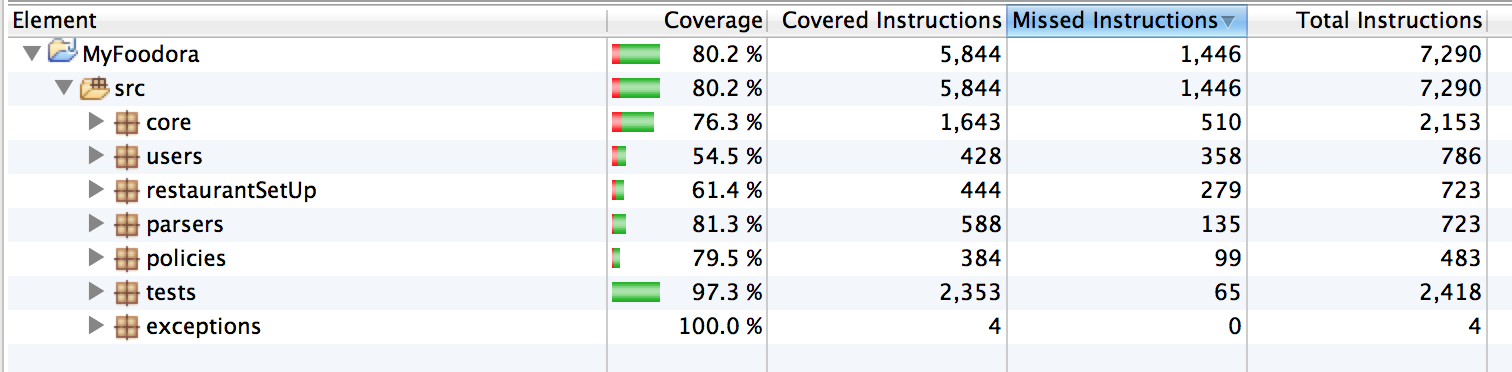
\includegraphics[scale=0.47]{./img/coverage_start.png} 
  \end{center}
  \caption{Code coverage results when using \textsc{EclEmma} for
  the first time.}
  \label{fig:coverage_first}
\end{figure} 

Next comes up the question to what extend the code has to be tested
while still being efficient.
It seems as ``\textit{the amount of testing necessary depends on a number of
factors}''~\cite{artimaHowMuchCoverage} that themselves depend
on how the code is written and what functions it implements.
Eventhough no particular goal for the coverage was set,
the plug-in allowed us to highlight the parts of the code that \emph{might not have been tested}
or that \emph{might be useless}. We finally achieved a $84.5\%$ code coverage after review (fig.~\ref{fig:coverage_end}).

\begin{figure}[h]
  \begin{center}
    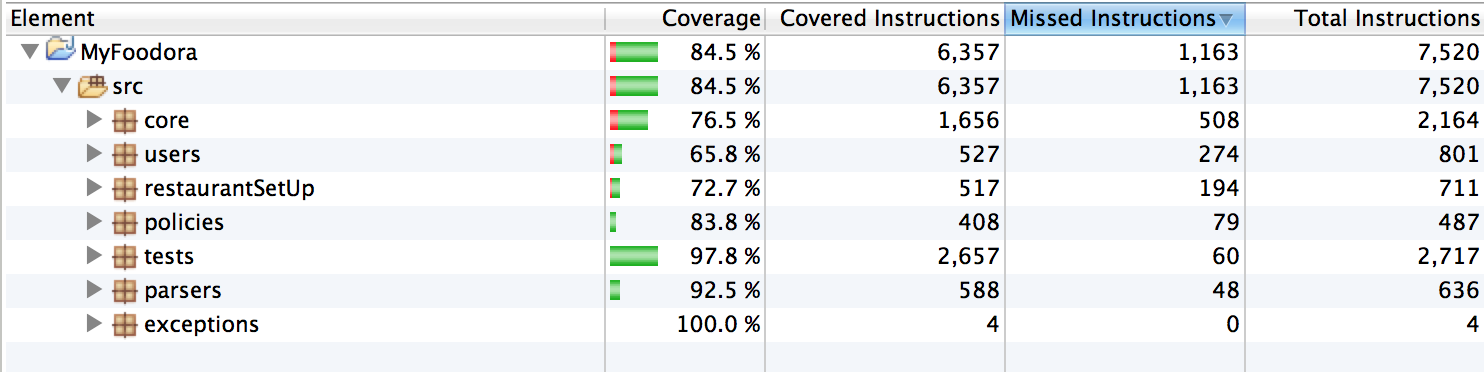
\includegraphics[scale=0.47]{./img/coverage_end.png} 
  \end{center}
  \caption{Code coverage results after review of
  tests using first results (fig.~\ref{fig:coverage_first}).}
  \label{fig:coverage_end}
\end{figure}

% section testing (end) 
\newpage
\section{User interface} % (fold)
\label{sec:user_interface}
This section describes in details the second part of the project.
First, an explanation will be made on the main design used in order
to have efficient command interpretation and execution.
Then will be described the effective implemenation
of the \emph{command line} user interface and the \emph{graphical} user inteface.


\subsection{Command line interface} % (fold)
\label{sub:command_line_interface}

Firstly, a note has to be made on the general choice of implementation
of the command line interface.
Following \textsc{Unix} command line style, one should be able to run
a command with multiple arguments in the following
style \lstinline|command -arg1_type arg1 -arg2_type arg2|.
In the \MyFoodora~case, it seems more adequate to have one syntax for each
command, being \lstinline|command <arg1> <arg2>|, which is proposed in 
the project requirements. The program will thus be able to give information
on the commands when needed and we expect the user to quickly remember 
the commands, as there are only few of them for each user type.
 
The choice of implementation described in the first paragraph
leads us to the use of an \lstinline|HashMap<String, Integer>| to
store the list of commands and their associated number of arguments,
as we only have \emph{one} number of arguments for one command,
except for the \lstinline|showTotalProfit| method which is handled
simply by using \lstinline|null| when no dates are given.

In terms of effeciency, using a parallel \lstinline|HashMap| to store
the commands names and their associated number of needed arguments
allows to check, if the given command name exists in $\mathcal{O}(1)$
time on average and in $\mathcal{O}(\log{n})$ on worst case~\cite{hashMap}.

\subsubsection{Separing interpretor from processor} % (fold)
\label{sub:separing_command_getter_and_command_processor}

Thinking about the design, we quickly realised the need to separate
the \emph{request} (ie. the given command) from its actual \emph{execution}.
This idea follows the open/close principle and has similar advantages
as design patterns (note that we discovered the \emph{command design pattern}~\cite{wiki:commandPattern} which is somewhat similar).
It indeed allows to easily change the behaviour of the program if
one wants to change the syntax of the commands (\emph{request} class)
or what a particular command does (\emph{execution} class).
This leads to the implementation of the \CommandLine~and
the \CommandProcessor~classes.

In order to make use of commands in an efficient way,
a \Command~class is designed.
It consists of a name and an array
of strings containing its arguments.
This allows the interpretor and processor to easily
communicate between themselves and with the real user.
The reader is advised to have a look at figure~\ref{fig:clui_uml}
containing the UML diagram of the relationship between
the three listed above classes.
One will notice the use of the Singleton pattern for
the \CommandProcessor~and \CommandLine.
This is justified by the fact that only one
of each will be required at the same time
and it does not created problems with \textsc{JUnit} tests
as those are made using concrete scenarios
generated by \texttt{.txt} files of commands.
% subsubsection separing_command_getter_and_command_processor (end)

\subsubsection{The \texttt{CommandLine} class} % (fold)
\label{ssub:the_commandline_class}
The \CommandLine~can be seen as the \emph{interpreter}. It will be the link
class between the real user and the system. It can either interpret commands
given directly as input with the \lstinline|launchFromInput()| method,
or listed in a \texttt{.txt} file with the \lstinline|launchFromFile| method.
Once a String, that should represent a command, is given to those methods,
they will call the \lstinline|getInputInfoAndProcessCmd| method whose
role is to check if the input
\begin{enumerate}
  \item corresponds to an existing command,
  \item has the ``$<>$'' argument declaration,
  \item has the right number of arguments associated with this command. 
\end{enumerate}
If one of those conditions is not satisfied, a message containing the
error description will be send back to the \lstinline|launch| method
which will print it out.
On the other hand, if the conditions are satisfied, the method
creates a new \Command~object and passes it to the \lstinline|processCmd|
method of its \CommandProcessor~attribute.
% subsubsection the_commandline_class (end)

\subsubsection{The \texttt{CommandProcessor} class} % (fold)
\label{ssub:the_commandprocessor_class}
The \CommandProcessor~can be seen as the \emph{executor}.
When its \lstinline|processCmd| receives a \Command~(which
is valid thanks to the \CommandLine),
it executes the behavior associated with the given command.
Its attributes mainly consist of the \Core~system,
as most of the method will need it and of 
a \lstinline|DishFactory| and a \lstinline|MealFactory|
that will be used to produce meals and dishes efficiently.

The methods of this class will mostly consists of translation
of user commands into \Core~commands.
It can easily be noticed that not all user commands are available in
the core but are directly applicable to the \lstinline|current_user|
of the core. For example when a courier wants to set his status
to \emph{avaible},
one simply executes \lstinline|core.getCurrent_courier().setAvailable(true)|.

The following is about how the \emph{creation of meals and orders} is handled. 
As we are required to create meals and orders
using multiple commands in the following pattern
\begin{enumerate}
  \item create a new \Meal~or \Order~giving basic information
  \item add dishes (resp. items) to \Meal~(resp. \Order)
  \item validate steps 2 and 3 by using a \lstinline|save| like function
\end{enumerate}
we used \emph{global} \lstinline|private| variables to handle this and therefore have an \lstinline|ArrayList<Meal>|
to store the potentials meals and an \Order~object.
Note that there is no need to store multiple orders, nor is there a need to give an order
name since a \Customer~will only place one order at a time
(see paragraph~\ref{par:order_creation_in_commandline} for a more detailed
explanation of order handling).

On the next page the reader will find the UML diagram of the
general structure of the CLUI and the listing~\ref{lst:commandline}
containing the application of the Singleton pattern of the
\CommandLine~class.
% subsubsection the_commandprocessor_class (end)
  
%%%%%%%%%%%%%%%%% SINGLETON WITH COMMANDLINE %%%%%%%%%%%%%%%%%
\begin{lstlisting}[caption=Singleton pattern with CommandLine class.,
   label=lst:commandline] 
private CommandLine() {
  cmd_processor = CommandProcessor.getInstance();
  command_list = ParseCommands.parseCommands("src/txtFILES/mf_commands.txt");
  for(Command cmd : command_list) {
    command_hm.put(cmd.getName(), cmd.getNb_args());
  }
}
private static class CommandLineHolder {
  private static final CommandLine INSTANCE = new CommandLine();
}
public static CommandLine getInstance() {
  return CommandLineHolder.INSTANCE;
}
\end{lstlisting}

\vspace{1cm}

\begin{figure}[H]
  \begin{center}
    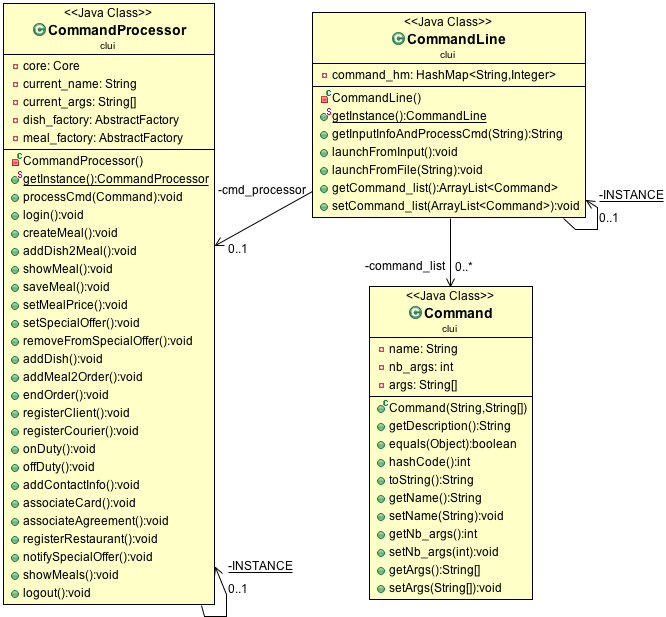
\includegraphics[scale=0.41]{./img/CLUI.png}
    \end{center}
  \caption{\umld of the command line user interface.}
  \label{fig:clui_uml}
\end{figure}

% subsection command_line_interface (end)


\newpage
\subsection{Graphical user interface} % (fold)
\label{sub:graphical_user_interface}

In order to connect the core to a \GUI~we used the \lstinline|java.swing|~package.
In the following, we will describe the general design structure of the gui package including 
its most important features. Then, we will give account of how errors and exceptions produced 
by the user are handled and how we tried to make the application as handy as possible. 
Lastly, we will discuss how we tested the \GUI~and how it should be used.

\subsubsection{General design} % (fold)
\label{ssub:general_design}

The \lstinline|gui|~package includes the following classes: 
\StFra,k\UserF,k\RestF,k\ManagF,k\CourF,k\CustF,k\lstinline|DisplayMealDish|,k\lstinline|LaunchGUI|~and 
\lstinline|StartFrameTest|. 
\lstinline|LaunchGUI| is there only to launch the gui (open the first frame), whereas 
\lstinline|StartFrameTest| takes care of testing some functionality.

We decides to build the \GUI~on two frames: One used for the registration and the loggin of a user
 (implemented via \StFra)
and the one for all functionality a user has as soon as he is logged in (implemented via  
\UserF, \RestF, \ManagF, \CourF, \CustF and \lstinline|DisplayMealDish|). 

To better understand how the frames are connected and how they are put in place by the classes, 
please take a closer look at figure~\ref{fig:start2user_uml} and figure~\ref{fig:userframe2users_uml}.
How exactly does the process work?
We decided to use a design pattern that is similar to the strategy design pattern, where as we use a 
the reference attribute \lstinline|CurrentLogInUser|~declared as a \UserF~to log in to different 
users (see listing~\ref{lst:login_user_GUI}). Thus the abstract class \UserF~forces each of the user 
classes to implement the \lstinline|getInstance()|~function to open up the individualized second frame. 
The advantages are: First, that we have a basic frame 
for all users that can individually be adapted and second, that we have saved the current user frame 
and can easily call it within the start frame. 
Whenever the log in button is succesfully clicked the first frame's visibility is set to 
\lstinline|false|~and the second frame opens. Logically, when the log out button is clicked the first 
frame's visibility is set to \lstinline|true|~and the second frame becomes invisible. 
This pattern allowed us to have a smooth and structured transition between the log in and register 
functionality used by every user and the individual user functionality all deriving from the same 
frame.

Next, we want to take a closer look of how we designed a clear and efficient structure for the 
different user's functionality by using \emph{nested classes}. Since each user can execute 
different functions, we decided to equip both the abstract \UserF~with some basic action classes to 
call setters and getters that are the same for all users as well as the user frames with more 
individualized action classes. These action classes provide action objects that were added to the 
respective menu bars of each user class frame and will execute their \textit{action} when clicked on. 
To can a better feeling of what we described in this paragraph, please take a look at the 
figure~\ref{fig:restaurantNestedClass_uml} and the listing~\ref{lst:nested_class_rest} both of which 
are using the \RestF~as an exemple. 
Every user frame has the basic menu items: Settings and Information as well as possible other 
individual ones. Clicking on a functional menu button will therefore trigger the functionality and 
execute the funtion. This design firstly gives a very clear overview of which functionality can be 
added to which menu bar item and is a very efficient way to handle many, but easy functionalities in 
a frame which is the case for our users (displaying and setting personal date as well as adding and 
removing dishes f.e.).

% subsubsection handling_of_the_gui (end)
\subsubsection{Handiness and Error handling} % (fold)
\label{ssub:handling_of_the_gui}

We tried to make the \GUI~as user friendly as possible by using a consistent and structured design 
and giving instructions when needed as partly already described above in 
section~\ref{ssub:general_design}. For that we will use buttons for the navigation in \StFra~as it 
has only two basic functionalities: log in and register. In the different user frames we also use 
buttons for basic navigation and the menu bar to execute the respective functionalities. 
For each menu bar action we added a little discription appearing when the mouse is held over the item 
as can be seen in the figure~\ref{fig:menuBarDescription}. Additionally we made sure that complicated 
functions like the ordering process of the client is explained in a pop up window (see figure~\ref{fig:instructionPopUp})
The handiness should be checked out by the user himself, but will also briefly demonstrated in a 
short video.

In the second part of this section, we quickly want to cover how we decides to handle bad user 
entries. When ever an exception is thrown due to a bad entry by the user, we catch it and will inform 
the user with the help of a pop up window. To get a better feeling for that, please take a look at 
figure~\ref{fig:wrongFormat}. We tried to make sure that the instructions are precise (giving clear 
instructions) and adapted for the different exceptions that can pop up.

% subsubsection general_design (end)
\subsubsection{Testing and Usage} % (fold)
\label{ssub:testing_and_usage}

Finally, we will explain how we tested and why we tested this way. 
When starting the \GUI~we weren't sure how we could test since all the correctness of the different 
functions was already tested in the first part of the project. Since it is not possible to test 
whether clicking on a button makes appear a certain frame or panel with \lstinline|JUnit|~tests, we 
found a way to implement so called \emph{bots} that will take control over mouse and be programmed to 
move on a certain position on the screen and click a button there. We implemented some tests for the 
\StFra~in the beginning to log in and register users, but we quickly realised that these tests will 
not be consistent if the layout of the frame changes (f.e. a button moving to a different position) 
and that there are to many possibilities to test. That is why, we decided to do most of the testing 
by hand afterwards. All the tests we implemented in the beginning can be found in 
\lstinline|StartFrameTest|~and you are invited to use them.

% subsubsection testing_and_usage

% subsection graphical_interface (end)


\newpage
\subsection{What differs from requirements ?} % (fold)
\label{sub:what_differs_from_requirements}

\paragraph{Meal creation in commandline} % (fold)
\label{par:meal_creation_in_commandline}
The first command line command which has been subject to a change
was the \lstinline|createMeal| command. Its new form is
\lstinline|createMeal <mealName> <mealType>|
which allows the restaurant to specify immediately which type of meal
he wants to create, it can either be a fullmeal or a halfmeal.
This prevents the system from failing in case the \lstinline|addDish2Meal|
is never called after this one.
The restaurant will immediately know which type of dishes he has to add
to the meal in order to stay consistent with the mealtype he gave. 
% paragraph meal_creation_in_commandline (end)

\paragraph{Order creation in commandline} % (fold)
\label{par:order_creation_in_commandline}
Then, we changed the \lstinline|createOrder| command. Its new form is
\lstinline|createOrder <restaurantName>|.
This is justified by the fact that naming an order by the customer
is of no use in our project nor in reality as the system
handles the assignement of an unique ID of the order.
One could argue that having an ordername allows to handle
multiple orders at the same time by the same customer,
which is indeed true but of no use either.
An order isn't restricted to a certain amount of dishes
or meals and thus a logged in customer will only
have to handle (create, add items to it and then end it)
the \emph{current order}.
% paragraph order_creation_in_commandline (end)

\paragraph{Adding an item to order with a quantity} % (fold)
\label{par:add_an_item_to_order_with_a_quantity}
A method called \lstinline|addNbItem2Order| has been added
in case the customer wants to order the same item more than once
and doesn't want to rewrite the same command multiple times.
This case scenario is useful in reality for group orders.
% paragraph add_an_item_to_order_with_a_quantity (end)

\paragraph{Merge of \texttt{endOrder} and \texttt{findDeliverer} methods} % (fold)
\label{par:merge_of_endorder_and_finddeliverer}
This choice is not about optimisation nor better representation of reality,
but only to how we implemented the \Core.
In the latter, we designed the order handling in a way that once an order
is placed, it is automatically treated, meaning the system finds a courier
following the delivery policy.
Finding the deliverer can thus only be made once an order is \emph{really}
added to the list of orders of the \Core.
Therefore, the \lstinline|endOrder| will take care of finding the courier
and showing it on screen, replacing the use of \lstinline|findDeliverer|.
% paragraph merge_of (end)

\paragraph{No need to specify the username for \texttt{onDuty}
and \texttt{offDuty} methods} % (fold)
\label{par:no_need_to_specify_the_username_for_lstinline_onduty_and_lstinline_offduty_methods}
As this function is used by the currently logged in courier,
our implementation of the core allows to keep track of the logged in user
and the latter doesn't need to specify his own username when changing his status.
% paragraph no_need_to_specify_the_username_for_lstinline_onduty_and_lstinline_offduty_methods (end)

\paragraph{Use of \texttt{showMenuItem} by any type of user} % (fold)
\label{par:use_of_lstinline_showmenuitem_by_any_type_of_user}
Instead of just being accessible to the mangare, showing all the menu
items can be done by any type of user.
This choice is motivated on one side because it is useful for both the customer
to have a list of what he can order and for the restaurant to remember what
is in its own menu, and on the other side because it is more realitic
as a menu card is something public that anyone can view.
% paragraph use_of_lstinline_showmenuitem_by_any_type_of_user (end)

% subsection what_differs_from_requirements (end)

% section user_interface (end) 
\newpage
\section{Results} % (fold)
\label{sec:results}

\subsection{Single command tests} % (fold)
\label{sub:single_command_tests}

\begin{table}[h]
  \begin{center}
    \begin{tabular}{|l|l|}
      \hline
      \textbf{Test file} & \textbf{Description}\\
      \hline
        \lstinline|testWrongCommandInput.txt|
        & Use non existing command,\\
        & command with no arguments, command with \\
        & wrong syntax and wrong number of arguments.  \\
        
        \lstinline|testLoginInput.txt|
        & \lstinline|login()| with known and unknown user. \\
        
        \lstinline|testRegisterRestaurantInput.txt|
        & \\
      \hline
    \end{tabular}
  \end{center}
  \caption{Description of all \lstinline|testXinput.txt| files contained
  in \texttt{eval/oneCommand/} folder.}
  \label{tab:clui_test}
\end{table}

% subsection single_command_tests (end)


% section results (end) 
\newpage
\section{Conclusion and further work} % (fold)
\label{sec:conclusion}

% section conclusion (end)
\newpage

\part*{Appendix}
\addcontentsline{toc}{part}{Appendix}
\appendix
\section{Code listing} % (fold)
\label{app:code_listing}

\lstset{basicstyle=\rm\footnotesize\ttfamily}

%%%%%%%%%%%%%%%%% OBSERVER PATTERN %%%%%%%%%%%%%%%%%
\begin{lstlisting}[caption=\emph{Observer} pattern for \texttt{Customer} and \texttt{Meal}.,
label=lst:observer]
public interface Observer {
  public void update(Meal specMeal, Restaurant r);
}

public class Customer extends User implements Observer {
  private boolean beNotified = true;
  public void update(Meal specMeal, Restaurant r){
    if (beNotified){
       System.out.println("[Customer UPDATE] " + ...);
} } }

public class Core {
  private void notifyCustomersOfSpecialOffer(){
    for(Customer cust : customerList){
      if (users.containsKey(cust.getUsername())){
        cust.update(current_restaurant);
} } } }
\end{lstlisting}

%%%%%%%%%%%%%%%%% STRATEGY PATTERN %%%%%%%%%%%%%%%%% strategy (fold)
\begin{lstlisting}[caption=\emph{Strategy} pattern for the \lstinline|DeliveryPolicy|.,
label=lst:strategy]
public interface DeliveryPolicy {
  public <G> ArrayList<Courier> howToDeliver(ArrayList<Courier> list, G g); 
}

public class FairOccupationDelivery implements DeliveryPolicy {
  private ArrayList<Courier> listCourier;
  
  public FairOccupationDelivery() {
  	super();
  	listCourier = new ArrayList<Courier>();
  }
  
  public <G> ArrayList<Courier> howToDeliver(ArrayList<Courier> list, G g) {
  	...
  }
}

public class FastestDelivery implements DeliveryPolicy {
  private ArrayList<Courier> courierListSorted;
  private ArrayList<Double> courierDistanceList;

  public FastestDelivery() {
  	super();
  	courierListSorted = new ArrayList<Courier>();
  	courierDistanceList = new ArrayList<Double>();
  }
 
  @Override
  public <G> ArrayList<Courier> howToDeliver(ArrayList<Courier> list, G g) {
  	...
  }
  
  public void getDistance(ArrayList<Courier> courierList, Address address) {
    ...
  }
  
}
\end{lstlisting}

\begin{lstlisting}[caption=Aggregation applied to the \Core~and its policies.,
  label=lst:aggregationCore]
public class Core{
    private DeliveryPolicy dPolicy;
    
    private TargetProfitPolicy tpPolicy;
    
    private SortPolicy sortPolicy;
}
  
\end{lstlisting}

% strategy (end)

%%%%%%%%%%%%%%%%% CURRENT USER SYSTEM %%%%%%%%%%%%%%%%% current_user (fold)
\begin{lstlisting}[caption=Application of the \texttt{current\_customer}
  concept to \texttt{getHistoryOfOrders}.,
  label=lst:historyOfOrders]
/**
 * Returns the history of orders of the current user, null if none is logged in.
 * @return an ArrayList of orders containing the orders of the current user
 */
public ArrayList<Order> getHistoryOfOrders() {
  if (current_customer != null){
    int temp_ID = current_customer.getID();
    ArrayList<Order> temp_cust_orders = new ArrayList<Order>();
    for(Order o : savedOrders){
      if (temp_ID == o.getCustomer().getID()){
        temp_cust_orders.add(o);
      }
    }
    return temp_cust_orders;
    
  } else {
    unauthorizedCommand();
    return null;
  }
}
\end{lstlisting}

%%%%%%%%%%%%%%%%% TEST EXAMPLES %%%%%%%%%%%%%%%%%
\begin{lstlisting}[caption=Example of a test using \texttt{assertEquals} with 2 decimal precision.,
  label=lst:test_total_income]
@Test
public void checkIfCalcTotalIncomeWorks() {
  make3orders();
  mf1.autoSetDateAfter();
  double totalIn = mf1.calcTotalIncome();
  //   3xdish1 : 3x8.3 = 24.9
  // + 2xdish2 : 2x6.35 = 12.7
  // + 1xdish3 : 1x16.85 = 16.85
  // + 3x(serviceFee + deliveryCost) : 3x2.5 = 7.5
  // ------------------------------------------------------
  // = 61.95
  assertEquals(totalIn, 61.95, 0.01);
  System.out.println("TEST chekcIfCalcTotalIncomeWorks : DONE\n");
}
\end{lstlisting}

%%%%%%%%%%%%%%%%% LOGIN / LOGOUT SYSTEM %%%%%%%%%%%%%%%%% 
% log-in\out (fold)
\begin{lstlisting}[caption=the main methods for the log in log out system.,
  label=lst:login]
public String logIn(String username){
  if (users.containsKey(username)){
    current_user = users.get(username);
    if (current_user instanceof Courier){
    	current_courier = (Courier) current_user;
    	output = "Successfully logged in as a Courier !";
    } else if (current_user instanceof Customer){
    	current_customer = (Customer) current_user;
    	output = "Successfully logged in as a Customer !";
    } else if (current_user instanceof Manager){
    	current_manager = (Manager) current_user;
    	output = "Successfully logged in as a Manager !";
    } else if (current_user instanceof Restaurant){
    	current_restaurant = (Restaurant) current_user;
    	output = "Successfully logged in as a Restaurant !";
    }
    current_user.checkMessages(); 
  }
  return output;
}
\end{lstlisting}

\begin{lstlisting}[caption=the main methods for the log in log out system.,
  label=lst:logout]
public void logOut(){
  current_user = null;
  current_courier = null;
  current_customer = null;
  current_manager = null;
  current_restaurant = null;
}
\end{lstlisting}

% log-in\out (end)

%%%%%%%%%%%%%%%%% PRICE ATTRIBUTES ORDER %%%%%%%%%%%%%%%%%

% attr_price (fold)
\begin{lstlisting}[caption=Implementation of different price quantities in \texttt{Order}.,
  label=lst:prices_order]
public class Order {
  ...
  private double profitFinal;
  private double priceInter;
  private double priceFinal;
  ...
  }
\end{lstlisting}
% attr_price (end)

%%%%%%%%%%%%%%%%% FASTEST DELIVERY %%%%%%%%%%%%%%%%%
% fastest deliv (fold)
 \begin{lstlisting}[caption=Pseudo java code of  fastest delivery method.,
   label=lst:fast_deliv_meth] 

@Override
ArrayList<Courier> howToDeliver(list of couriers, Address) {
  ...
  list of distances = getDistance(list of couriers, Address);	
  sorted courier list = IntStream.range(0, amount of members in list of distances)
    .mapToObj(i -> new CourierDistance(list of couriers(i), list of distances(i)))
    .sorted(Comparator.comparingDouble(CourierDistance -> distance of CourierDistance))
    .map(CourierDistance -> Courier of CourierDistance())
    .collect(Collectors.toList());
  		
  return sorted courier list;
}
  
\end{lstlisting}

% fastest deliv (end)

%%%%%%%%%%%%%%%%% CREATE FACTORY %%%%%%%%%%%%%%%%%
\begin{lstlisting}[caption= Factory producer for \texttt{Dish} and \texttt{Meal}.,
label=lst:createFactory]
public static AbstractFactory getFactory(String choice){
		if (choice.equalsIgnoreCase("DISH")){
			return new DishFactory();
		} else if (choice.equalsIgnoreCase("MEAL")){
			return new MealFactory();
		}
		return null;
	}
\end{lstlisting}

%%%%%%%%%%%%%%%%% CREATE MEAL %%%%%%%%%%%%%%%%%
\begin{lstlisting}[caption=\emph{MealFactory} to create \texttt{Meal}.,
label=lst:mealCreator]
public Meal getMeal(String mealType, String mealName){
		if (mealType.equalsIgnoreCase("FULLMEAL")){
			return new FullMeal(mealName);
		} else if (mealType.equalsIgnoreCase("HALFMEAL")){
			return new HalfMeal(mealName);
		} 
		return null;		
	}
\end{lstlisting}

%%%%%%%%%%%%%%%%% SETFULLMEAL %%%%%%%%%%%%%%%%%
\begin{lstlisting}[caption=Set method to add \texttt{Dish} to \texttt{Meal}.,
label=lst:SetFullMeal]
public void setFullMeal(Starter starter, MainDish mainDish, Dessert dessert) {
		
		getListOfDish().add(starter);
		getListOfDish().add(mainDish);
		getListOfDish().add(dessert);
		
		String type = "standard";
			
		if((starter.getType() == mainDish.getType()) && (mainDish.getType()==dessert.getType()))
			type = mainDish.getType();
		setType(type);
	}
\end{lstlisting}

%%%%%%%%%%%%%%%%% ADD MEAL %%%%%%%%%%%%%%%%%
\begin{lstlisting}[caption=\emph{Add method} for \texttt{Meal}.,
label=lst:addMeal]
public void addMeal(Meal meal) {
		listOfMeal.add(meal);
	}
\end{lstlisting}

%%%%%%%%%%%%%%%%% TREAT ORDER %%%%%%%%%%%%%%%%%
\begin{lstlisting}[caption=Method to treat \texttt{Order} of \texttt{Core}.,
label=lst:treatOrder]
private void treatNewOrders(){ 
	
		Order = latest order in list;
		list of couriers = DeliveryPolicy.howToDeliver(list of couriers, address);
			
		while(courier of order is filled OR there are no couriers left) { 
			courier = first courier according to list;
			courier reply to order;
			remove courier of list
		}

		if there are no couriers left { --> no order 
		} else {
			set final price of order (= price of meals or dishes + service fee);
			save order;
			inform system that order has been saved;
			inform restaurant to prepare order;
			inform customer of execution of order and final price 
		}
}
\end{lstlisting}

%%%%%%%%%%%%%%%%% PLACE ORDER %%%%%%%%%%%%%%%%%
\begin{lstlisting}[caption=Method to place an \texttt{Order} of \texttt{Core}.,
label=lst:placeOrder]
public void placeNewOrder(Order order){
		if (current_customer != null){
			this.receivedOrders.add(order);
			update(this.current_customer,"Your order has succesfully been placed.");
			treatNewOrders();
		} else {
			unauthorizedCommand();
		}
	}
\end{lstlisting}

\lstset{basicstyle=\rm\small\ttfamily}
% section code_listing (end)

\newpage
\section{UML class diagrams characteristics} % (fold)
\label{sec:uml_class_diagrams_characteristics}

% section uml_class_diagrams_characteristics (end)
\newpage
\section{Workload division} % (fold)
\label{app:who_did_what}
One way to verify what is presented in the below table or 
just to get more details of how the work has been executed
is to have a look at our project public repository on \textsc{GitHub}
\begin{center}
  \url{https://github.com/jdewasseige/IS1220-project}
\end{center}

% \vspace{3\baselineskip}
The work has been globally divided as described in table~\ref{tab:who_did_what},
where student A is John de Wasseige and student B is Patrick von Platen.

\begin{table}[H]
  \begin{center}
    \begin{tabular}{|l|c|}
      \hline
      \textbf{Task} & \textbf{Student}\\
      \hline
      \Dish~and \Meal~factory pattern &              A\\
      User &              A\\
      Courier &              B\\
      Customer &              A\\
      Manager &              A\\
      Restaurant &              A\\
      Parsers &  A + B\\
      Tests during coding &  A + B\\
      Code coverage review &  A\\
      Target profit policy &              B\\
      Delivery policy &              B\\
      Sort shipped order &              B\\
      Fidelity plan policy &             B\\
      Report intro, design and testing  &             A\\
      Report background, implementation  &             B\\
      Report conclusion &  A + B\\
      UML diagrams &                           A\\
      \User~management in \Core &             A\\
      \Order~management in \Core &             B\\
      Javadoc &  A + B\\
      \hline
    \end{tabular}
  \end{center}
  \caption{Workload division for the main functionnalities of
  the first part of the project. Student A is John de Wasseige
  and student B is Patrick von Platen.}
  \label{tab:who_did_what}
\end{table}

% section who_did_what (end)
\newpage

\addcontentsline{toc}{part}{References}
\nocite{*}
\hypersetup{urlcolor=black}
\printbibliography
%\newpage

\end{document}